
\section{Vector Addition Exercises}

\begin{comment}
This lab was originally written by Ted Bunn, sometime between 2002 and 2004.  Introduced into the regular 131 lab manual in 2015 by Matt Trawick, with some tweaking of Latex formatting: blame all typos on Matt.  Besides the stated ``objectives'' below, this lab does a nice job of walking students through using a = delta v / delta t in the limit of delta t getting small.

\end{comment}

Name \rule{2.0in}{0.1pt}\hfill{}Section \rule{1.0in}{0.1pt}\hfill{}Date \rule{1.0in}{0.1pt}

\textbf{Objectives}

To add and subtract velocity vectors graphically and algebraically, and discover something about centripetal acceleration in the process.


\textbf{Apparatus}
\begin{itemize} \itemsep1pt
\item ruler
\item protractor 
\end{itemize}

\bigskip

{\bf 1}.
Suppose that two forces pull on the same object.  The first force has
a strength of 75.0 N and pulls in a direction $30.0^\circ$ from the $x$
axis.  The second force has a strength of 65.0 N and pulls in a direction 
$160^\circ$ from the $x$ axis.  (For this exercise, all you need
to know about forces is that they obey the rules for vector addition.
The N stands for ``newton,'' which is the standard metric unit of force.)

(a) Draw a careful diagram of these two vectors, and use it to figure out
what single force would be equivalent to the combination of these two.
Use a ruler and protractor, and choose a scale for your diagram so that
the diagram takes up a large portion of a single page.

(b) Now add the two vectors using 
trigonometry instead
of graphical addition.  Are the results consistent?

\vfil\vfil

(c) What single force would cancel out the effects of the original two?  That
is, what third force, when added to those two, gives a total of zero?
Give both magnitude and direction.  (After you've answered the
previous question, this one can be answered very quickly.)

\vfil\eject


{\bf 2}.  Suppose a car is driving counterclockwise around a circular track as shown
below.  The radius of the track is 250 m, and the car is traveling
at a steady speed of 45.0 m/s.\footnote{Professional driver on closed
course.  Do not attempt this yourself!}

\begin{figure}[h]
\centerline{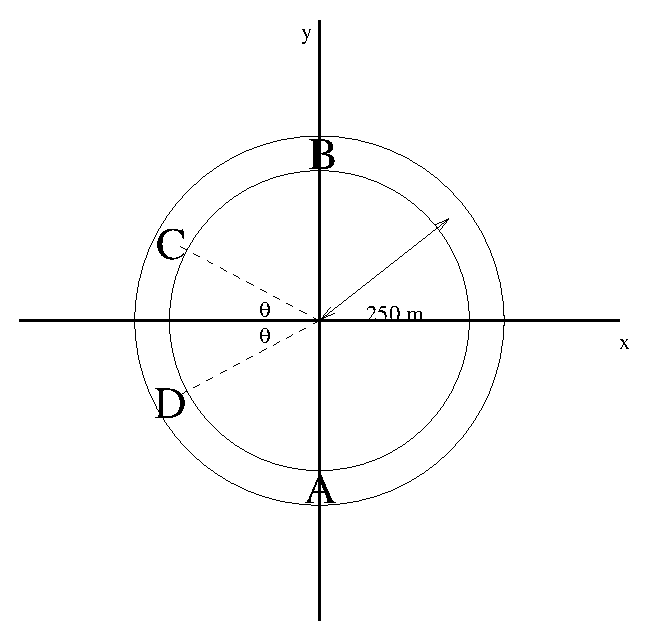
\includegraphics{vectors/veclabfig.eps}}
\end{figure}

(a) Give the magnitude and direction of the vector $\Delta{\bf v}_{AB}$
that represents the change in velocity between the moment when the
car is at point A and the moment when the car is at point B.  (Note:
the velocity at any given moment is a vector whose magnitude is the
car's speed at that moment and whose direction is the direction that
the car is going at that instant.  $\Delta{\bf v}$ still means
final velocity minus initial velocity, but since the velocities are
now vectors, you must use vector subtraction.)

\vfil

(b) Determine the elapsed time between the moment the car is at point A
and point B.  Use this, together with the answer to part (a), to determine
the car's average acceleration over this time interval.  (Give both magnitude
and direction.)  {\bf Note:} Acceleration is still defined the same
way it was before: $\overline{\bf a}={\Delta {\bf v}\over\Delta t}$.
The only difference is that $\Delta{\bf v}$ is now a vector.


\vfil\eject

(c) Determine the change in velocity $\Delta {\bf v}_{CD}$ between the
car's velocity at point C and at point D.  Assume that the angle $\theta$
is $10^\circ$.  (Suggestion: First draw a picture of the two
velocity vectors and use it to decide which way
$\Delta{\bf v}$ is going to point.  Then determine the relevant
components ($x$ or $y$) of the two velocity vectors.)

\vfil

(d) Determine the elapsed time between the moment the car is at
point C and the moment it is at point D, and use this to figure out
the car's acceleration over the time interval from C to D.
(Suggestion: In order to do this, decide what fraction of a complete
circuit the car is making.  How long does it take to make a complete circuit?)

\vfil\eject

(e) Repeat parts (c) and (d), but this time, assume the angle $\theta$ is 
$1^\circ$.

\vfil

(f) Do you think the average accelerations you have determined make a good
approximation to the instantaneous acceleration?

\vskip 0.8in

(g) What would the magnitude and direction of the instantaneous acceleration
at point A be?

\vskip 0.8in\eject

